\chapter{Estabilidade de Sistemas Não Lineares}\label{cap_EstSistNaoLin}


\section{Introdução}

A estabilidade é o desempenho mínimo de todo sistema de controle, por isso é a primeira propriedade a ser verificada antes que se inicie o projeto do controlador para este sistema. Neste trabalho, mais especificamente neste capítulo, nos despenderemos em determinar a estabilidade de pontos de equilíbrio de sistemas não lineares. O método a ser utilizado para a determinação da estabilidade dos pontos de equilíbrio dos sistemas em estudo consiste na chamada Estabilidade de Lyapunov, proposta em 1892  pelo matemático e engenheiro russo que dá nome a esta teoria \cite{bookkhalil:2003}. A teoria de Estabilidade de Lyapunov investiga o comportamento da resposta do sistema em torno do ponto de equilíbrio situado na origem do plano de estados, de forma tal que permite não apenas determinar se o ponto de equilíbrio é estável, assintoticamente estável ou instável, mas, caso se conclua que o ponto de equilíbrio equivale a uma dentre as duas primeiras possibilidades supracitadas, permite também obter a estimativa da região no plano de estados para a qual a estabilidade do ponto é valida. A região para a qual o ponto de equilíbrio é um ponto estável ou assintoticamente estável é dita região de atração do ponto de equilíbrio, a qual será objeto de estudo do capítulo \ref{cap_RegAtrac}. Neste capítulo, portanto, vamos nos ater a verificar a estabilidade para o ponto de equilíbrio do sistema situado na origem do plano de estados segundo proposto por Lyapunov.

\section{Estabilidade de Lyapunov}

Antes de definir Estabilidade de Lyapunov, mais especificamente Estabilidade de Lyapunov via LMIs, que será a abordagem utilizada neste trabalho, será feita uma breve contextualização de como se dá o uso de funções de Lyapunov para o estudo de estabilidade de um ponto de equilíbrio na origem. Para tanto, será utilizado o exemplo do pêndulo simples.

\subsection{Estabilidade de um ponto de equilíbrio}

Antes de definirmos de forma sistemática a estabilidade de Lyapunov, vamos retomar uma discussão iniciada no Capítulo \ref{cap_ModelagemSisNaoLinearesporFuzzyTS}. Na Seção \ref{subsec_phasePortrait} vimos que um ponto de equilíbrio é caracterizado conforme o comportamento da resposta do sistema a partir de pontos iniciais próximos a este. Se as respostas permanecem próximas ao ponto de equilíbrio, este é dito estável, caso contrário, é instável. O ponto de equilíbrio é assintoticamente estável se, quando o tempo tende ao infinito, a resposta do sistema tende ao ponto de equilíbrio.

Considerando um sistema não linear autônomo, ou seja, independente do tempo, constituído de equações de estado não forçadas descrito por

\begin{equation}\label{sist_autonomo}
\mathbf{\dot{x} = f(x)}
\end{equation}

Onde o domínio de $\textbf{f}$ é tal que $\textbf{f}: C \rightarrow I\!R^n$, com $C \subset I\!R^n$, tal que $\textbf{0} \in D$. Supondo também que $\textbf{x = 0}$ sempre será o ponto de equilíbrio do sistema da equação \ref{sist_autonomo}, a definição de estabilidade de um ponto de equilíbrio pode ser reescrita, segundo descrito por \cite{bookkhalil:2003}, conforme apresentado a seguir.

\begin{defn} (Khalil, 2003)\cite{bookkhalil:2003}\label{def:pontoEquilibrio}
 O ponto de equilíbrio \textbf{x = 0} de \ref{sist_autonomo} é
\begin{itemize}
\item estável se, para cada $\varepsilon > 0$, existe $\delta = \delta(\varepsilon) > 0$ tal que
\begin{equation*} ||\textbf{x}(0)|| < \delta \Rightarrow ||\textbf{x}(t)|| < \varepsilon, \forall t \geq 0
\end{equation*}
\item instável, se não for estável;
\item assintoticamente estável se for estável e $\delta$ puder ser escolhido tal que
\begin{equation*}||\textbf{x}|| <\delta \Rightarrow \lim_{x\to\infty} \textbf{x}(t) = 0
\end{equation*}
\end{itemize}
 \end{defn}

Em outras palavras, a Definição \ref{def:pontoEquilibrio} diz que, para qualquer valor de $\varepsilon$ escolhido, tem-se um valor de $\delta = \delta(\varepsilon)$ tal que uma trajetória começando em uma vizinhança $\delta$ da origem nunca deixará a vizinhança $\varepsilon$. A Figura \ref{fig:epsilon_delta} exemplifica esta definição. A região delimitada pela linha azul contendo a origem equivale a $\delta$, esta região contém todas as possibilidades de pontos iniciais tais que as respostas do sistema jamais deixem a região $\varepsilon$ contendo a origem, representada pela cor vermelha na figura.

\begin{figure}[htbp]
	\centering
	\includegraphics[width=10cm]{epsilon_delta}
	\caption{Região $\varepsilon$, em vermelho, e $\delta$, em azul, utilizadas para definir a estabilidade do ponto de equilíbrio na origem}
	 \label{fig:epsilon_delta}
\end{figure}

Vale lembrar, que, como visto no capítulo anterior, caso o ponto de equilíbrio do sistema não seja na origem, este pode ser deslocado para a origem sem que haja perda de generalidade. Para tanto, basta utilizar o método de mudança de variável.

Para ilustrar as properiedades de estabilidade de um ponto de equilíbrio segundo a Definicção \ref{def:pontoEquilibrio}, será analisado o modelo de um pêdulo \cite{bookkhalil:2003}, o qual é é descrito no exemplo a seguir.

\begin{example} [Pêndulo simples] Considere o pêndulo simples mostrado na Figura \ref{fig:pendulo}, onde $L$ é o comprimento da haste e $m$ é a massa do prumo na ponta da haste. Assuma que a haste é rígida e que tem massa igual a zero e que o pêndulo é livre de balanço no plano vertical. $\theta$ é o ângulo entre a haste e o eixo vertical. A haste do pêndulo se move num círculo de raio L. 

\begin{figure}[htbp]
	\centering
	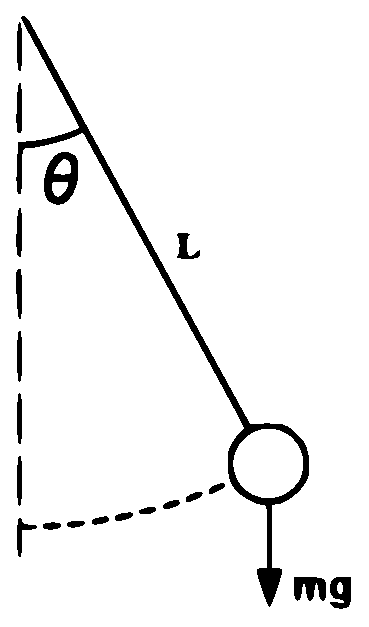
\includegraphics[width=4cm, height=6cm]{pendulum}
	\caption{Pêndulo simples}
	 \label{fig:pendulo}
\end{figure}

A equação de movimento do pêndulo pode ser obtida utilizando-se a segunda lei de Newton, considerando que há uma componente de força gravitacional igual a $mg$ agindo sobre o prumo, onde $g$ é a aceleração da gravidade. Além disso, há um componente de atrito $k$, que é proporcional \`{a} valocidade do prumo. Assim obtém-se a equação de movimento na direção tangencial, conforme segue.
\begin{equation*} mL\ddot{\theta} = -mg\sin\theta - kL\dot{theta}
\end{equation*}
Assumindo $x_1 = \theta$ e $x_2 = \dot{\theta}$, o modelo de estados do pêndulo passa a ser
\begin{equation*}
\begin{cases}\dot{x_1} = x_2\\\dot{x_1} = -\dfrac{g}{L} \sin(x_1) - \dfrac{k}{m} x_2
\end{cases}
\end{equation*}

Os pontos de equilíbrio do pêndulo simples são obtidos fazendo-se $\dot{x_1} = \dot{x_2} = 0$ e resolvendo para $x_1$ e $x_2$. Logo, os pontos de equilíbrio são $(x_1,x_2) = (0,0)$ e $(x_1, x_2) = (\pi,0)$. O retrato de fase do sistema para valores arbitrários dos parâmetros é mostrado na Figura \ref{fig:pendulo_retrato_fase}, onde a Figura (a) equivale ao retrato de fase considerando-se o atrito diferente de zero e a Figura (b) assume atrito igual a zero.

\begin{figure}[htbp]
	\centering
	\subfigure[ref1][Retrato de fase considerando atrito diferente de zero]{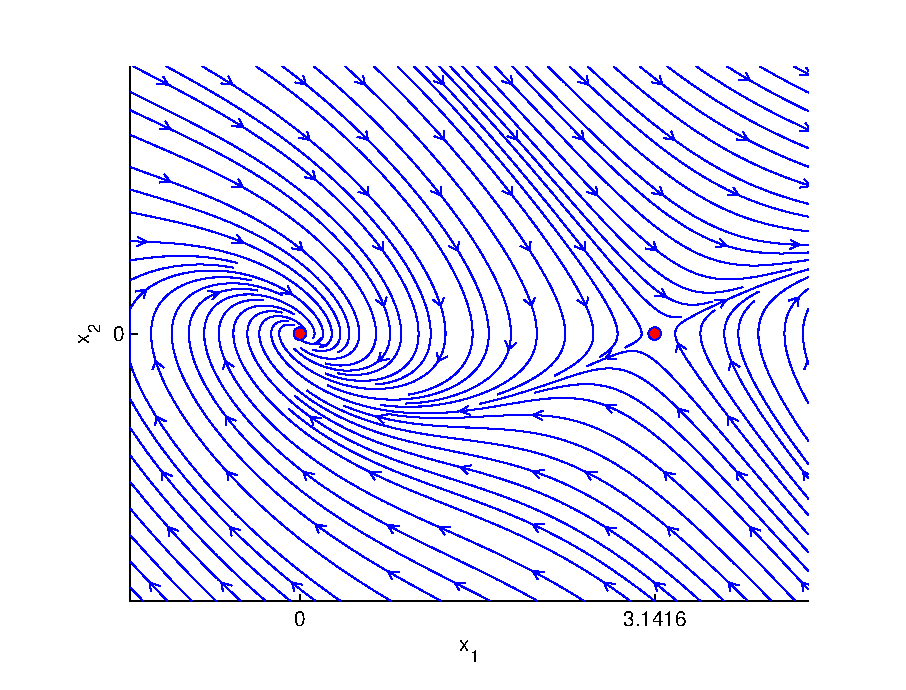
\includegraphics[width=7cm]{pendulum_phase_portrait}}
	\qquad
	\subfigure[ref2][Retrato de fase considerando atrito igual a zero]{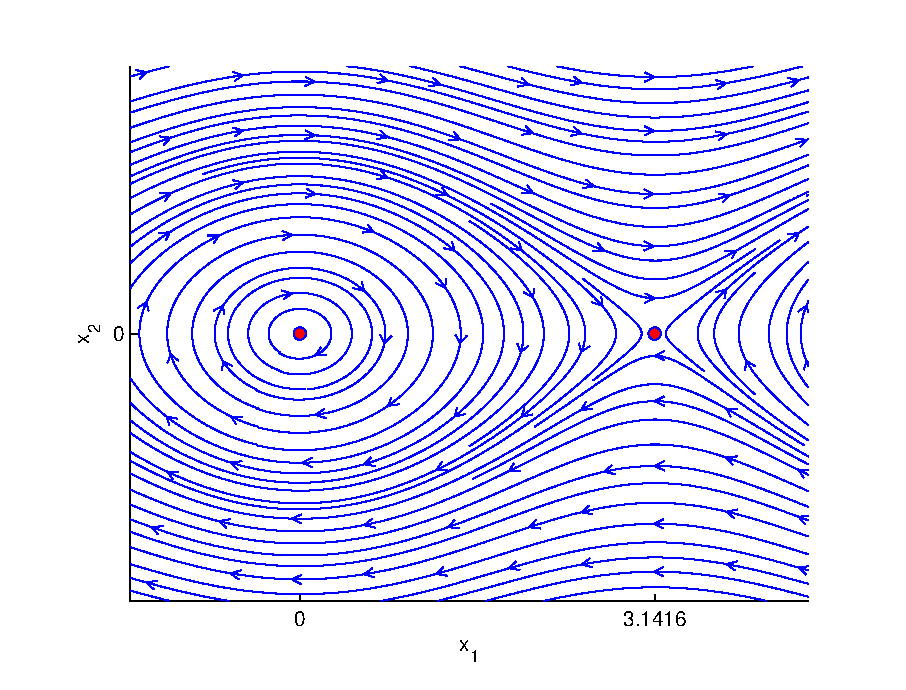
\includegraphics[width=7cm]{pendulum_phase_portrait_k_0}}
	\caption{Retrato de fase do pêndulo simples com atrito diferente de zero e com atrito igual a zero}
	\label{fig:pendulo_retrato_fase}
\end{figure}

\end{example}\label{ex:pendulo_simples}

Neste exemplo do pêndulo simples, quando o atrito é nulo, as trajetórias na vizinhança do ponto de equilíbrio $(0,0)$ são órbitas fechadas. Assim, escolhendo-se um ponto inicial suficientemente perto deste ponto de equilíbrio, é garantido que as trajetórias permanecerão sempre em torno deste, de forma que a relação $\varepsilon-\delta$ necessária para a estabilidade é satisfeita.

No caso em que o atrito é considerado, o ponto de equilíbrio localizado na origem, além de as trajetórias na vizinhança manterem-se próximas a este, estas também tendem ao ponto de equilíbrio quando o tempo tende ao infinito. Mais uma vez, verifica-se que  a origem do plano de estados e sua vizinhança satisfaz a relação $\varepsilon-\delta$ necessária para a estabilidade e, desta vez, também verifica-se que este ponto é assintoticamente estável. Já o ponto de equilíbrio $(\pi, 0)$ se comporta como um ponto de sela e, em ambos os caso, em que se assume o atrito diferente de zero e, em seguida, igual a zero, não se é possível obter uma região $\delta$ tal que as respostas estejam sempre contidas em uma região $\varepsilon$, pois sempre haverá uma trajetória que sairá desta região.

A verificação da estabilidade de pontos de equilíbrio por meio do retrato de fase é uma técnica bastante limitada, pois somente pode ser aplicada para sistemas de, no máximo, terceira ordem. E, ainda, tem-se a desvantagem de ser difícil de se observar o comportamento das trajetórias de resposta ao redor do ponto de equilíbrio para sistemas de terceira ordem, como visto no exemplo \ref{ex:droop_UFSM}.

Como uma tentativa de se obter de forma generalizada e objetiva conclusões sobre a estabilidade dos pontos de equilíbrio do sistema, pode-se utilizar conceitos de energia \cite{bookkhalil:2003}. Neste exemplo, portanto, considera-se que a energia total do sistema é obtida da soma da energia potencial e da energia cinética, com a referência da energia potencial escolhida como sendo zero quando as variáveis de estado são iguais a zero. Para o atrito nulo, não há dissipação de energia, logo, a energia total do sistema é constante durante o movimento, ou seja, a variação de energia é igual a zero ao longo das trajetórias do sistema ($dE/dt = 0$). O fato de a energia total $E$ ser constante mesmo com o passar do tempo para qualquer valor das variáveis de estado $\textbf{x}$ permite obter uma curva correspondente a um contorno fechado ao redor da origem do plano de estados de raio $r = E$, podendo-se constatar a estabilidade do ponto de equilíbrio $(0,0)$.

Quando se considera a influência do atrito, a variação da energia total $E$ é negativa ($dE/dt \leq 0$), ou seja, a energia se dissipa ao longo tempo. Quando o tempo tende ao infinito, a energia se dissipa totalmente, porém, para cada instante de tempo, a energia total equivale a um valor constante cada vez menor, revelando diferentes contornos que satisfazem a condição para estabilidade, até que o raio da curva tende a zero, revelando que o ponto é assintoticamente estável.

Desta maneira, verifica-se que apenas examinando a variação da energia ao longo das trajetórias do sistema é possível determinar a estabilidade do ponto de equilíbrio. O que Lyapunov propõe em sua teoria de estabilidade é que diversas outras funções, além da energia total do sistema, podem ser usadas, de forma semelhante ao que foi ilustrado acima, para determinar a estabilidade de um ponto de equilíbrio. A próxima seção traz a definição do modelo de determinação de estabilidade proposto por Lyapunov via LMIs.

\subsection{Estabilidade de Lyapunov via Desigualdades Matriciais Lineares (LMIs)}

Antes de iniciar a discussão sobre Estabilidade de Lyapunov nesta seção, será primeiramente introduzido o conceito de função convexa e, em seguida, de Desigualdades Matriciais Lineares (LMIs, do inglês \textit{Linear Matrix Inequalities}), uma vez que as soluções propostas neste trabalho utilizam sistemas convexos e as LMIs são ferramentas poderosas para resolver de forma eficiente este tipo de sistema.

Um conjunto $S$ definido no $\rm I\!R^{n}$ é dito convexo se contém qualquer segmento reta formada a partir de dois pontos quaisquer pertencentes a este conjunto, isto é , $x, y \in S,\quad\lambda,\mu\geq0,\quad\lambda+\mu=1\Rightarrow\lambda x +\mu y\in S$ \cite{inproc:hin:2004}. A Figura \ref{fig:sets_exmples} ilustra um conjunto convexo e de um conjunto não convexo, respectivamente.

\begin{figure}[htbp]
	\centering
	\subfigure[ref1][Conjunto Convexo]{
\includegraphics[width=5cm]{convex_set_example}}
	\qquad
	\subfigure[ref2][Conjunto não convexo]{
\includegraphics[width=5cm]{nonconvex_set_example}}
	\caption{Conjuntos convexo e não convexo}
	\label{fig:sets_exmples}
\end{figure}

Uma função $f$ é dita convexa se seu domínio é convexo e para todo $x \in \textbf{dom} f, \theta \in [0, 1]$ vale a seguinte relação.
\begin{equation*}
f(\theta x+(1-\theta)y) \leq f(x)+(1-\theta)f(y)
\end{equation*}

Uma LMI é uma desigualdade matricial do tipo $F(g) > 0$, definida no domínio $\rm I\!R^{m}$ e com imagem em $\rm I\!R^{q \times q}$, simétrica e afim nas variáveis de busca, representadas pelo vetor $g$. Uma representação genérica de uma LMI é dada por
\begin{equation}\label{eq:rep_lmi}
F(g) = F_0+\sum_{i = 1}^{m}g_iF_i>0\quad g = \begin{bmatrix}g_1\\\vdots\\g_m\end{bmatrix}
\end{equation}
em que $F_i = F_i' \in \rm I\!R{q \times q}$ são matrizes dadas e $g_i$ são variáveis escalares a serem determinadas de forma a satisfazer a desigualdade, quando existe uma solução para tal, ou seja, quando a LMI é factível. Dificilmente uma LMI aparecerá na forma gerérica da Equação \ref{eq:rep_lmi}, no entanto, a conversão para este formato é feita internamente pelos pacotes de resolção de LMI aqui utilizados.

Definido o conceito de LMI, estamos agora aptos a discutir sobre a análise de estabilidade proposta por Lyapunov via LMIs. O teorema de estabilidade de Lyapunov caracteriza a estabilidade de um sistema através de uma função $V(x)$, chamada função de Lyapunov, a qual deve satisfazer algumas condições, que serão apresentadas mais a frente. A principal vantagem atrelada ao teorema de Lyapunov é o fato de este poder ser aplicado para determinação da estabilidade de um sistema $\dot{\textbf{x}} = f(\textbf{x})$ sem que se precise resolvê-lo. Por outro lado, não há um método sistemático para se obter funções de Lyapunov, sendo responsabilidade do projetista determiná-las.

Considere $V(x)$ uma função contínua, diferenciável definida no domínio $D \subset \rm I\!R^{n}$, tal que em $D$ esteja contida a origem. A variação de $V(x)$ ao longo das trajetórias do sistema $\dot{x} = f(x)$ é dada por

\begin{equation*}
\dot{V}(x) = \sum_{i = 1}^{n} \frac{\partial V}{\partial x_i}\dot{x}_i = \sum_{i = 1}^{n} \frac{\partial V}{\partial x_i} f_i(x) = \begin{bmatrix}\frac{\partial V}{\partial x_1},&\hdots,&\frac{\partial V}{\partial x_n}\end{bmatrix}\begin{bmatrix}f_1(x)\\\vdots\\f_n(x)\end{bmatrix} = \frac{\partial V}{\partial x}f(x)
\end{equation*}

Logo, $\dot{V}(x)$ é dependente da equação do sistema e, portanto, será diferente para cada sistema \cite{bookkhalil:2003}. E, se $\dot{V}$ for negativa, então $V$ diminui ao longo do tempo da solução do sistema. Assim, o teorema de Lyapunov é enunciado, conforme segue.

\begin{theorem}[Khalil, 2003 \cite{bookkhalil:2003}]\label{th:lyap_stability}
 Seja $x = 0$ um ponto de equilíbrio do sistema não linear autônomo $\dot{x} = f(x)$ e seja $D \subset \rm I\!R^{n}$ um domínio contendo $x = 0$. Seja $V: D \rightarrow \rm I\!R$ uma função diferenciável contínua tal que
\begin{equation}\label{eq:def_V}
V(0) = 0\quad\text{e}\quad V(X) > 0\quad\text{em}\quad D - \{0\}
\end{equation}
\begin{equation}\label{eq:def_dot_V_stable}
\dot{V}(x) \leq 0\quad\text{em}\quad D
\end{equation}
então, $x = 0$ é estável. Além disso, se
\begin{equation}\label{eq:def_dot_V_assymp_stable}
\dot{V}(x) < 0\quad\text{em}\quad D - \{0\}
\end{equation}
então $x = 0$ é assintoticamente estável.
\end{theorem}

As inequações enunciadas no Terorema \ref{th:lyap_stability} são conhecidas como Inequações de Lyapunov. Estas inequações equivalem \`{a}s primeiras LMIs utilizadas para analisar a estabilidade de sistemas dinâmicos, podendo ser resolvidas analiticamente, a partir de um conjunto de equações lineares. As Inequações de Lyapunov são cada vez mais utilizadas  em aplicações em problemas práticos, importantes e difíceis na engenharia de controle.

A função de Lyapunov $V(x)$, utilizada para a determinação da estabilidade de sistemas aparece na forma de funções quadráticas, conhecida como forma quadrática \cite{bookboydl:1994}.

Uma forma quadrática equivale a uma função $\nu(x)$ definida no espaço $\rm I\!R^{n}$ tal que
\begin{equation}\label{eq:forma_quadr}
\nu(x) = \sum_{i = 1}^{n}\sum_{j = 1}^{n}p_{ij}x_ix_j,\quad p_{ij} = p_{ji}
\end{equation}
Em que $x_i$ e $x_j$ são componentes quaisquer do vetor de estados $x$ e $p_{ij}$ são constantes. O exemplo a seguir apresenta uma forma quadrática simples.

\begin{example}\label{ex:forma_quadr}
\begin{equation*}
V(x) = 9x_1^2+3x_1x_2+7x_1x_2+6x_2^2 = 9x_1^2+10x_1x_2+6x_2^2 = 9x_1^2+5x_1x_2+5x_1x_2+6x_2^2
\end{equation*}
\end{example}

É válido também dizer que toda forma quadrática pode ser representada em termos matriciais a partir de uma matriz simétrica cujos elementos são as constantes $p_{ij}$. Assim o Exemplo \ref{ex:forma_quadr} é reescrito na forma
\begin{equation*}
V(x) = \begin{bmatrix}x_1\\x_2\end{bmatrix}'\begin{bmatrix}9&5\\5&6\end{bmatrix}\begin{bmatrix}x_1\\x_2\end{bmatrix} = x'Px
\end{equation*}

Sabendo que toda matriz simétrica possui autovalores reais, a função $\nu(x) = x'Px$ é positiva para todo $x \neq 0$ se, e somente se, os autovalores de $P$ forem todos positivos. Quando satisfeita esta condição, a matriz $P$ é dita positiva definida ($P > 0$) \cite{bookboydl:1994}.

\subsection{Definição do problema}\label{subsec:contextualization}

Considere o sistema não linear
\begin{equation}\label{eq:nonlinear_system_cap_stability}
\dot{\mathbf{x}} = f(\mathbf{x}(t))
\end{equation}
tal que a origem é um ponto de equilíbrio, ou seja, $f(\textbf{0}) = \textbf{0} \in \rm I\!R^p$, em que $p$ é a ordem do sistema, isto é, a quantidade de variáveis de estado. Considere, ainda, a representação fuzzy T-S exata obtida pelo método de aproximação por não linearidade de setor, como visto no capítulo anterior, tal que
\begin{equation}\label{eq:fuzzy_TS_system_cap_stability}
\dot{\mathbf{x}} = A(\mathbf{\alpha) x}(t)
\end{equation}
onde $A(\alpha) \in \rm I\!R^{p \times p}, \forall x(t) \in \chi$, em que $\chi$ é uma região no espaço de estados incluindo a origem, para a qual o sistema está definido. Além disso,
\begin{equation}\label{eq:A_alpha_cap_stability}
A(\alpha) = \sum_{i = 1}^{r} \alpha_i(z)A_i
\end{equation}
Desta maneira, define-se $\alpha(z) = [\alpha_1, ..., \alpha_r] \in \Lambda_r$, em que
\begin{equation}\label{lambda_r}
\Lambda_r = \{\alpha \in \rm I\!R^r | \sum_{i = 1}^{r} \alpha_i(z) = 1,\quad \alpha_i(z) \geq 0\}
\end{equation}
e $z(t)$ são as variáveis de premissa dependentes dos estados, o que equivale a $z(x(t))$. O domínio de validade $\chi$ do modelo fuzzy Takagi-Sugeno pode ser dado pela seguinte representação poliédrica limitada, com $0 \subset \chi$,
\begin{equation}\label{eq:chibk}
\chi = 
\{ x \in \rm I\!R^{p} | b_k'x \leq 1, k = 1, ..., q \leq p\}
\end{equation}
em que os elementos $b_k \in \rm I\!R^{p}, k = 1, ..., m$ são definidos na modelagem fuzzy Takagi-Sugeno do sistema. A região $\chi$ também pode ser modelada em termo de seus $v$ vértices, tal que
\begin{equation}\label{eq:chixk}
\chi = 
co\{ x^1, x^2, ..., x^v \}
\end{equation}
em que $x^{i}$ são vértices da região politópica do domínio $\chi$ de validade do modelo.
\begin{observation}Seja dada a região do plano de estados para a qual o sistema é definido, como $|x_i| < \sigma_i$, então esta região pode ser representada como um conjunto convexo $\chi$ dado como a interseção de um número finito de semi-espaços fechados limitados, tal que
	\begin{equation*}
	\chi = \{x | Nx \leq \Phi\}
	\end{equation*}
	A configuração de $\chi$ descrita acima é conhecida como politopo, que é um poliedro limitado \cite{inproc:MPT:2006}. É possível concluir, a partir da definição vista, que todo politopo representa uma configuração convexa e compacta (limitada e fechada).
	
	Os termos $b_k$ da forma normalizada da representação de um politopo por semi-espaços vista na equação \ref{eq:chibk} são obtidos conforme segue.
	\begin{equation*}
	b_k' = \dfrac{N(k, :)}{\Phi(k)},\quad k = 1, 2, ...
	\end{equation*}
	Uma das propriedades fundamentais de um politopo é que este pode ser descrito em função de seus vértices \cite{inproc:MPT:2006}, de forma que
	\begin{equation}\label{eq:chixk_simplex}
	\chi = \{x \in \rm I\!R^{n} | x = x(\gamma) = \sum_{k = 1}^{v} \gamma_i(x)x^k,\quad 0 \leq \gamma_k \leq 1,\quad \sum_{k = 1}^{v} \gamma_k(x) = 1\}
	\end{equation}
	em que $x^i$ é o i-ésimo vértice de $\chi$ e $v$ é o número total de vértices de $\chi$. É fácil notar que a representação por vértices apresentada nesta Observação equivale \`{a} representação descrita na Equação \ref{eq:chixk}.
	
	O exemplo a seguir ilustra como obter a representação por semi-espaços e a representação por vértices de um politopo.
	\begin{example}\label{exe:rep_politopica}
		Considere um sistema com três estados $x_1$, $x_2$ e $x_3$ tais que $|x_1| \leq 2$ e $|x_2| \leq 3$ e $\forall x_3$ (livre).
		
		A representação politópica por semi-espaços é dada por
		\begin{equation*}
		\begin{bmatrix}1&0&0\\0&1&0\end{bmatrix} = \begin{bmatrix}x_1\\x_2\\x_3\end{bmatrix} \leq \begin{bmatrix}2\\3\end{bmatrix}
		\end{equation*}
		Logo,
		\begin{equation*}
		\begin{bmatrix}\dfrac{1}{2}&0&0\end{bmatrix}x \leq 1\Rightarrow b_1'x\leq 1
		\end{equation*}
		\begin{equation*}
		\begin{bmatrix}0&\dfrac{1}{3}&0\end{bmatrix}x \leq 1\Rightarrow b_2'x\leq 1
		\end{equation*}
		Já a representação por vértices é obtida como sendo
		\begin{equation*}
		\chi = co\begin{Bmatrix}
		\begin{bmatrix}-2\\-3\\x_3\end{bmatrix},\begin{bmatrix}-2\\3\\x_3\end{bmatrix},\begin{bmatrix}2\\-3\\x_3\end{bmatrix},\begin{bmatrix}2\\3\\x_3\end{bmatrix}
		\end{Bmatrix}
		\end{equation*}
	\end{example}
\end{observation}

\subsection{Análise de estabilidade}\label{subsec:stabilily_analysis}

Neste trabalho será investigada a estabilidade quadrática de sistemas. Para tanto, serão utilizadas funções de Lyapunov na forma quadrática, tal que
\begin{equation}\label{eq:Lyap_quadr}
V(x) = x'Px
\end{equation}

Desta forma, para o sistema ser assintoticamente estável, sabe-se que, além de $P$ ser definida positiva, deve ser satisfeita a desigualdade $\dot{V}(x) < 0$. $\dot{V}(x)$, considerando a forma quadrática apresentada na Equação \ref{eq:Lyap_quadr}, é obtida conforme segue.
\begin{equation}\label{eq:V_dot}
\dot{V}(x) = \dot{x}'Px + x'\dot{P}x + x'P\dot{x} < 0
\end{equation}

Assumindo um sistema na forma $\dot{x} = Ax$, a equação \ref{eq:V_dot} pode ser rescrita como
\begin{equation}\label{eq:V_dot_A}
\dot{V}(x) = x'A'Px + x'\dot{P}x + x'PAx = x'(A'P + PA + \dot{P})x 
\end{equation}
Portanto, o sistema ser exponencialmente estável, isto é, os autovalores da matriz $A$ possuem parte real estritamente negativa se, e somente se, existir uma matriz $P$ simétrica definida positiva tal que \cite{bookboydl:1994}
\begin{equation}\label{eq:est_quadr_PA}
A'P + PA + \dot{P} < 0
\end{equation}

A matriz $P$ pode ser invariante no tempo ou variante no tempo, este segundo caso implica que $P$ será dependente dos estados do sistema, uma vez que estamos trabalhando com sistemas autônomos. Assim, no caso em se considera $P$ independente dos estados do sistema, a respectiva derivada será igual a zero, podendo a equação \ref{eq:est_quadr_PA} ser reduzida para 
\begin{equation}\label{eq:metodo_Lyapunov}
A'P + PA < 0
\end{equation}

Assumindo $P$ independente dos estados, pode-se enunciar o seguinte Teorema para a análise de estabilidade de sistemas fuzzy Takagi-Sugeno com a matriz $P$ da função de Lyapunov constante.
\begin{theorem}[Boyd, 1994 \cite{bookboydl:1994}]\label{th:est_boyd} Se existe uma matriz P = P' > 0 tal que
	\begin{equation}\label{eq:LMIs_est_met_3}
	A(\alpha)'P + PA(\alpha) < 0
	\end{equation}
	para todo $\alpha \in \Lambda_r$, então a origem do sistema (\ref{eq:fuzzy_TS_system_cap_stability}) é assintoticamente estável.
\end{theorem}

No caso em que $P$ é dependente dos estados do sistema, é possível obter resultados menos conservadores para a análise de estabilidade do ponto de equilíbrio na origem de um determinado sistema. Assim, a estabilidade de sistemas fuzzy Takagi-Sugeno para $P$ dependente dos estados do sistema, mais precisamente $P$ dependente das funções de associação de cada vértice do modelo fuzzy T-S, será o principal objeto de estudo deste trabalho. 

Antes de enunciarmos o teorema correspondente ao resultado principal deste trabalho, vamos enunciar um teorema que visa determinar a condição de estabilidade para sistemas fuzzy T-S também utilizando a teoria de estabilidade de Lyapunov via LMIs. Este teorema foi proposto por (Mozelli, Palhares, Sousa e Mendes, 2009) \cite{MPSM:2009}. Nele verifica-se a estabilidade para sistemas definidos em uma região simétrica limitada do plano de estados. Para tanto, é proposto o seguinte teorema \cite{MPSM:2009}, para o qual deve-se considerar a forma quadrática alternativa para $V(x) = x'\sum_{i = 1}^{r}(\alpha_iP_i)x$, em que $\alpha_i$ são as funções de associação de cada vértice $A_i$ do sistema fuzzy T-S obtido pelo método não linearidade de setor local.

\begin{theorem}[Mozelli, Palhares, Sousa e Mendes, 2009 \cite{MPSM:2009}]\label{th:theorem_6}
	Assuma que $|\dot{\alpha}_k| \leq \Phi_k$, $k \in \{1, \ldots, r \}$. O sistema fuzzy Takagi-Sugeno \ref{eq:fuzzy_TS_system_cap_stability} é estável se as seguintes LMIs são satisfeitas
	\begin{equation}\label{eq:theorem6_LMI1}
	P_i=P_i'\succ0,\quad i \in \{1, \ldots, r\},
	\end{equation}
	\begin{equation}\label{eq:theorem6_LMI2}
	P_i+X\succeq0,\quad i \in \{1, \ldots, r\},
	\end{equation}
	\begin{equation}\label{eq:theorem6_LMI2}
	\overset{-}{P}_{\Phi}+\dfrac{1}{2}(A_i'P_j+P_jA_i+A_j'P_i+P_iA_j)\preceq 0,\quad i\leq j.
	\end{equation}
	onde $j=1,\hdots ,r$, $\overset{-}{P}_{\Phi} = \sum_{k = 1}^{r}\Phi_k(P_k+X)$, $\Phi_k$ são grandezas escalares e $X$ é qualquer matriz simétrica de dimensão apropriada.
\end{theorem}

Em outras palavras, o que o Teorema \ref{th:theorem_6} estabelece é que, dado o modelo fuzzy Takagi-Sugeno obtido para uma região local $C$, e seja $\Phi_k$ a região limitada pela variação da função de associação $\alpha_k$ do modelo fuzzy T-S, então achar uma solução para as LMIs deste teorema consiste em garantir que o sistema é estável para a região contida por $\dot{\alpha}_k\leq\Phi_k$. Observe que há métodos mais eficientes de se levar em consideração o limitante da derivada das funções de pertinência conforme apresentado por (Tognetti, Oliveira e Peres, 2011) \cite{article:TOP:11b}.

\section{Resultado principal}\label{sec:resultado_principal}

Nesta seção é proposto um Teorema que utiliza funções de Lyapunov fuzzy de modo a se encontrar condições de estabilidade mais relaxadas do que outras apresentadas na literatura.

Portanto, considere a função de Lyapunov
\begin{equation}\label{eq:lyapunov_func_p_alpha}
V(x) = x'P(\alpha)x, \quad \alpha = \alpha(z(x)), \quad x = x(t)
\end{equation}
em que
\begin{equation}\label{eq:p_alpha}
P(\alpha) = \sum_{i = 1}^{r} \alpha_i(z)P_i\qquad P_i = P_i' \in \rm I\!R^{n \times n}
\end{equation}
Então,
\begin{equation*}
\dot{V}(x) = \dot{x}'P(\alpha)x + x'P(\alpha)\dot{x} + x'\dot{P}(\alpha)x
\end{equation*}
Substituindo $\dot{x}$ na equação acima pela Equação \ref{eq:fuzzy_TS_system_cap_stability} e rearranjando os termos, tem-se
\begin{equation*}
\dot{V}(x) = x'(A(\alpha)'P(\alpha) + P(\alpha)A(\alpha))x + x'\dot{P}(\alpha)x
\end{equation*}
O último termo da equação anterior, $ x'\dot{P}(\alpha)x$, pode ser reapresentado substituindo-se $\dot{P}(\alpha)$ pela Equação \ref{eq:p_alpha}. Assim,
\begin{equation}\label{eq:xT_P_x}
\begin{array} {lcl}
x'\dot{P}(\alpha)x & = & x'(\sum_{i = 1}^{r} \alpha_i(z)P_i)x\\
& = & x'(\dot{\alpha}_1P_1 + ... + \dot{\alpha}_rP_r)x\\
& = & x'\begin{bmatrix}P_1x&...&P_rx\end{bmatrix}\begin{bmatrix}\dot{\alpha}_1\\\vdots\\\dot{\alpha}_r\end{bmatrix}\\
& = & x'\begin{bmatrix}P_1x&...&P_rx\end{bmatrix}\dot{\alpha}(z)
\end{array}
\end{equation}
Observe que a derivada da função de pertinência $\alpha(z)$ em relação a $x$ é uma função de $x$ dado que a variável premissa $z$ é função de $x$. Dessa forma, pode ser aplicada a  modelagem por não linearidade de setor descrita na Seção \ref{subsec:sector_nonlinearuty_modeling} para descrever $\nabla_x  \alpha(z)$ por meio de uma combinação convexa, como mostrado a seguir.
\begin{equation*}
\dot{\alpha}(z) = J(\theta)\dot{x},
\end{equation*}
com
\begin{equation*}
\dot{\alpha}(z) = \begin{bmatrix}\dot{\alpha}_1\\\vdots\\\dot{\alpha}_r\end{bmatrix}\qquad
\dot{x} = \begin{bmatrix}\dot{x}_1\\\vdots\\\dot{x}_r\end{bmatrix}
\end{equation*}
\begin{equation*}
J(\theta) = \nabla_x\alpha(z) = \sum_{i = 1}^{\vartheta}\theta_i(x)J_i,\quad \theta\in\Lambda_{\vartheta}
\end{equation*}
Portanto, a Equação \ref{eq:xT_P_x} passa a ser
\begin{equation*}
x'\dot{P}(\alpha)x = x'\begin{bmatrix}P_1x&\hdots&P_rx\end{bmatrix}J(\theta)A(\alpha)x
\end{equation*}
Este termo também é bilinear em $x$. Desta maneira, $x$ pode ser substituído por sua representação politópica em função de seus respectivos vértices, conforme a Equação (\ref{eq:chixk_simplex}). Assim,
\begin{equation*}
\begin{array} {lcl}
x'\dot{P}(\alpha)x & = & x'\begin{bmatrix}P_1x(\gamma)&\dots&P_rx(\gamma)\end{bmatrix}J(\theta)A(\alpha)x\\
& = &  x'Q(\gamma)J(\theta)A(\alpha)x
\end{array}
\end{equation*}
onde
\begin{equation*}
Q(\gamma) = \sum_{k = 1}^{v}\gamma_k\begin{bmatrix}P_1x^k& \hdots &P_rx^k\end{bmatrix}
\end{equation*}

Sabendo que $\sum_{i = 1}^{r}\alpha(z) = 1$, então $\sum_{i = 1}^{r}\dot{\alpha}(z) = 0$, podemos reescrever $\sum_{i = 1}^{r}\dot{\alpha}(z)$ conforme segue.
\begin{equation*}
\begin{array} {lcl}
\sum_{i = 1}^{r}\dot{\alpha}(z) & = & \begin{bmatrix}1&\hdots&1\end{bmatrix}\begin{bmatrix}\dot{\alpha}_1\\\vdots\\\dot{\alpha}_r\end{bmatrix}\\
 & = & \textbf{1}'\dot{\alpha}\\
& = &\textbf{1}'J(\theta)\dot{x}\\
& = &\textbf{1}'J(\theta)A(\alpha)x = 0,\quad\textbf{1} = \begin{bmatrix}1&\hdots&1\end{bmatrix}'
\end{array}
\end{equation*}
Portanto, finalmente, temos que a derivada da função de Lyapunov fuzzy, conforme segue.
\begin{equation}\label{eq:dot_V_fuzzy}
\begin{array}{rcr}
\dot{V}(x) = x'(A(\alpha)'P(\alpha) + P(\alpha)A(\alpha) + Q(\gamma)J(\theta)A(\alpha))x,\\
\textbf{1}'J(\theta)A(\alpha)x = 0
\end{array}
\end{equation}
Considere agora o a versão reduzida do Lema de Finsler, enunciado a seguir.
\begin{lemma}[Lema de Finsler - versão reduzida] Considere $\omega \in \rm I\!R^{n}, D \in \rm I\!R^{n \times n}$ e $B \in \rm I\!R^{m \times n}$  com $rank(B) < n$. Então as afirmações a seguir são equivalentes.
\begin{enumerate}
\item $\omega'D\omega < 0,\quad\forall\omega\neq0,\quad B\omega = 0$
\item $\exists X \in \rm I\!R^{n \times m} : D+XB + B'X <0$
\end{enumerate}
\label{lem:finsler_short_version}\end{lemma}
Portanto, se aplicarmos o Lemma \ref{lem:finsler_short_version} no resultado obtido em \ref{eq:dot_V_fuzzy}, em que $\omega' D \omega = \dot{V}(x)$ $\dot{V}(x) < 0$, sendo $\dot{V}(x)$ obtido na Equação \ref{eq:dot_V_fuzzy}, e $B = \textbf{1}'J(\theta)A(\alpha)$, então $\dot{V}(x) < 0$ será válido se
\begin{equation}\label{eq:dot_V_fuzzy_finsler}
A(\alpha)'P(\alpha) + P(\alpha)A(\alpha) + Q(\gamma)J(\theta)A(\alpha) + X(\alpha)\textbf{1}'J(\theta)A(\alpha) + A(\alpha)'J(\theta)'\textbf{1}X(\alpha)' < 0
\end{equation}
ou\footnote{$He\{M\}$ significa $He\{M\} = M + M'$}
\begin{equation}\label{eq:dot_V_fuzzy_finsler_He}
He\{(P(\alpha) + X(\alpha)\textbf{1}J(\theta))A(\alpha)\} + Q(\gamma)J(\theta)A(\alpha) < 0,\quad \forall\alpha\in\Lambda_n, \forall\theta\in\Lambda_{\vartheta}, \forall\gamma\in\Lambda_{\nu}.
\end{equation}

Desta maneira, podemos propor o seguinte teorema.

\begin{theorem}[Proposto]\label{th:main_result}
 Se existem matrizes $P(\alpha) = P(\alpha)' > 0$ e $X(\alpha)$ tais que
\begin{equation}\label{eq:th1_stability}
A(\alpha)'P(\alpha) + P(\alpha)A(\alpha) + Q(\gamma)J(\theta)A(\alpha) + X(\alpha)\textbf{1}'J(\theta)A(\alpha) + A(\alpha)'J(\theta)'\textbf{1}X(\alpha)' < 0
\end{equation}
para todo $\alpha \in \Lambda_r$, $\theta \in \Lambda_{\vartheta}$ e $\gamma \in\Lambda_{\nu}$ , então o sistema \ref{eq:fuzzy_TS_system_cap_stability} é assintoticamente estável.
\end{theorem}

\begin{proof}[Prova do Teorema \ref{th:main_result}] Seja dado
\begin{equation*}
He\{P(\alpha)A(\alpha) + X(\alpha)\textbf{1}J(\theta)A(\alpha)\} + Q(\gamma)J(\theta)A(\alpha) < 0
\end{equation*}
Pré e pós multiplicando por $x$, tem-se
\begin{equation}\label{eq:proof_1}
He\{x'P(\alpha)A(\alpha)x + x'X(\alpha)\textbf{1}J(\theta)A(\alpha)x\} + x'Q(\gamma)J(\theta)A(\alpha)x < 0
\end{equation}
Como $A(\alpha)x = \dot{x}$, $J(\theta)\dot{x} = \dot{\alpha}$ e $\textbf{1}'\dot{\alpha} = \sum_{i = 1}^{r}\dot{\alpha}_i = 0$, então a expressão \ref{eq:proof_1} é equivalente a
\begin{equation*}
He\{x'P(\alpha)A(\alpha)x\} + x'Q(\gamma)\dot{\alpha} < 0
\end{equation*}
Como $Q(\gamma) = \begin{bmatrix}P_1x(\gamma)&\hdots&P_rx(\gamma)\end{bmatrix}$, quando $x \in \chi$, tem-se
\begin{equation*}
x'P(\alpha)A(\alpha)x + x'A(\alpha)'P(\alpha)x + x'(\sum_{i = 1}^{r}\dot{\alpha}_iP_i)x < 0
\end{equation*}
Portanto, $\dot{V}(x) < 0$.
\end{proof}

\section{Exemplos Numéricos}

Todas as rotinas desenvolvidas para obtenção dos resultados deste trabalho foram implementadas no MATLAB, versão  8.2.0.701 (R2013b), utilizando-se as toolboxes YALMIP \cite{Lofberg2004} e SEDUMI \cite{sedumi:2002}. Além disso, o pacote ROLMIP \cite{inproc:ROLMIP:2016} foi usado para implementar o conjunto de LMIs de dimensão finita.

\subsection{Exemplo sistema de segunda ordem}\label{sec:ex2_JPJ12_again}

Nesta seção será utilizado o Exemplo \ref{example_LPJ12} apresentado no capítulo anterior de forma a se analisar a estabilidade do ponto de equilíbrio deste sistema. Para este fim, serão utilizados os Teoremas \ref{th:est_boyd} e \ref{th:theorem_6} encontrados na literatura, além do Teorema \ref{th:main_result}. Posteriormente, os resultados obtidos a partir destes três teoremas serão comparados para se verificar qual gera condições menos conservadoras. O procedimento a ser adotado para a comparação consiste em, primeiramente, verificar se o sistema é estável para a região politópica para a qual o sistema é definido considerando $\lambda = 20$, que é o valor assumido para este parâmetro até o momento. Em seguida, serão verificados os valores mínimos e máximos de $\lambda$ para os quais o sistema permanece estável, para qualquer região contida em $\chi$.

 O exemplo em questão será reapresentado para facilitar o entendimento do leitor.

\begin{example}\label{ex:example2_LPJ12_non_linear_system}
Considere o Exemplo \ref{example_LPJ12}, em que se tem um sistema de segunda ordem não linear descrito pelas equações a seguir
\begin{equation}\label{eq:ex2_LPJ12_non_linear}
\begin{cases}\dot{x}_1 = -2x_1 + 4x_2
\\-(1 + \dfrac{\lambda(1 - \sin(x_1))}{2})x_1 - 2x_2\end{cases},\qquad \lambda = 20
\end{equation}
com $x_1$ e $x_2$ pertencentes à região do plano de estados descrita por $C = \{x \in \rm I\!R^n | |x| \leq \pi/2\}$. Para este mesmo valor de $\lambda$, o modelo fuzzy Takagi-Sugeno deste sistema foi obtido no Exemplo \ref{ex:LPJ12_fuzzyTS}, resultando nos vértices e funções de pertinência mostrados a seguir.
\begin{equation*}
\alpha_1(z(t)) = \dfrac{1+\sin(x_1(t))}{2}\qquad \alpha_2(z(t)) = 1 - \alpha_1(z(t))
\end{equation*}
\begin{equation*}
A_1 = \begin{bmatrix}-2&4\\-1&-2\end{bmatrix}\qquad A_2 = \begin{bmatrix}-2&4\\-(1+\lambda)&-2\end{bmatrix}
\end{equation*}
\end{example}

\subsubsection{Método 1: (Boyd, 1994 \cite{bookboydl:1994}) Função de Lyapunov com $P$ constante e Teorema \ref{th:est_boyd}}

Este primeiro método compreende a utilização da dinâmica fuzzy Takagi-Sugeno na função de Lyapunov, com $P$ constante. O parâmetro $A$ da função de Lyapunov passa a ser dependente das funções de associação, ou seja, $A = A(\alpha)$. Desta forma, as LMIs necessárias para a garantir a estabilidade são apresentadas no Teorema \ref{th:est_boyd}.

No capítulo anterior foi obtido o modelo fuzzy Takagi-Sugeno do sistema não linear utilizado nesta seção. Esta modelagem foi apresentada no Exemplo \ref{ex:LPJ12_fuzzyTS} e o resultado é reapresentado nesta seção. Conforme mostra a Equação \ref{eq:A_alpha} e sabendo que o modelo fuzzy deste exemplo possui apenas dois vértices, $A(\alpha)$ é obtido conforme segue.
\begin{equation*}
A(\alpha) = \alpha_1 \begin{bmatrix}-2&4\\-1&-2\end{bmatrix}+ \alpha_2 \begin{bmatrix}-2&4\\-(1+\lambda)&-2\end{bmatrix}
\end{equation*}

Ao se resolver as LMIs \ref{eq:LMIs_est_met_3}, verificou-se que o ponto de equilíbrio situado na origem não é estável para para a toda a região $C$, limitada pelas variáveis de estado. Assim, reduziu-se a região gradativamente obtendo, para cada nova região, um novo modelo fuzzy T-S, limitado para este novo setor local, até que se obteve a nova região para a qual o ponto de equilíbrio é estável.

Desta forma, obteve-se que o sistema é estável em torno do ponto de equilíbrio situado na origem, e assumindo-se $\lambda = 20$, apenas para regiões no espaço de estados menores ou iguais a $0.46\cdot C$, em que C é a região delimitada pelos limites das variáveis de estado, descrita na Seção \ref{sec:ex2_JPJ12_again} como sendo $C = \{x \in \rm I\!R^n | |x| \leq \pi/2\}$. Em outras palavras, a estabilidade só é garantida, segundo o Método 1, assumindo $\lambda = 20$ para modelos fuzzy dentro da região $C_1 = \{x \in \rm I\!R^n | |x| \leq 0.46\pi/2\}$

Para a região $C$, foi feita a busca pelos valores máximos e mínimos de $\lambda$ para os quais se verifica que o sistema é estável para este método. Assim foram obtidos os seguintes valores
\begin{align*}\lambda_{min_1} &= -1.9000\\\lambda_{max_1} &=9.6000\end{align*}

\subsubsection{Método 2: (Mozelli, Palhares, Sousa e Mendes, 2009 \cite{MPSM:2009}) Função de  Lyapunov com $P$ dependente das funções de pertinência e limitante simples das derivadas do Teorema \ref{th:theorem_6}}

Este método permite verificar a condição de estabilidade para sistemas definidos em uma região simétrica, como é o caso de $C$ no exemplo utilizado nesta seção, por meio do Teorema \ref{th:theorem_6}.

. Para tanto, é proposto o seguinte teorema \cite{MPSM:2009}, para o qual deve-se considerar a forma quadrática alternativa para $V(x) = x'\sum_{i = 1}^{r}(h_iP_i)x$, em que $\alpha_i$ são as funções de associação de cada vértice $A_i$ do sistema fuzzy T-S construído pelo método não linearidade de setor local.

A Figura \ref{fig:hk_phik} ilustra graficamente a relação entre $\Phi_k$ e $\dot{\alpha}_1$ e $\dot{\alpha}_2$ para o Exemplo \ref{sec:ex2_JPJ12_again}.

\begin{figure}[htbp]
	\centering
	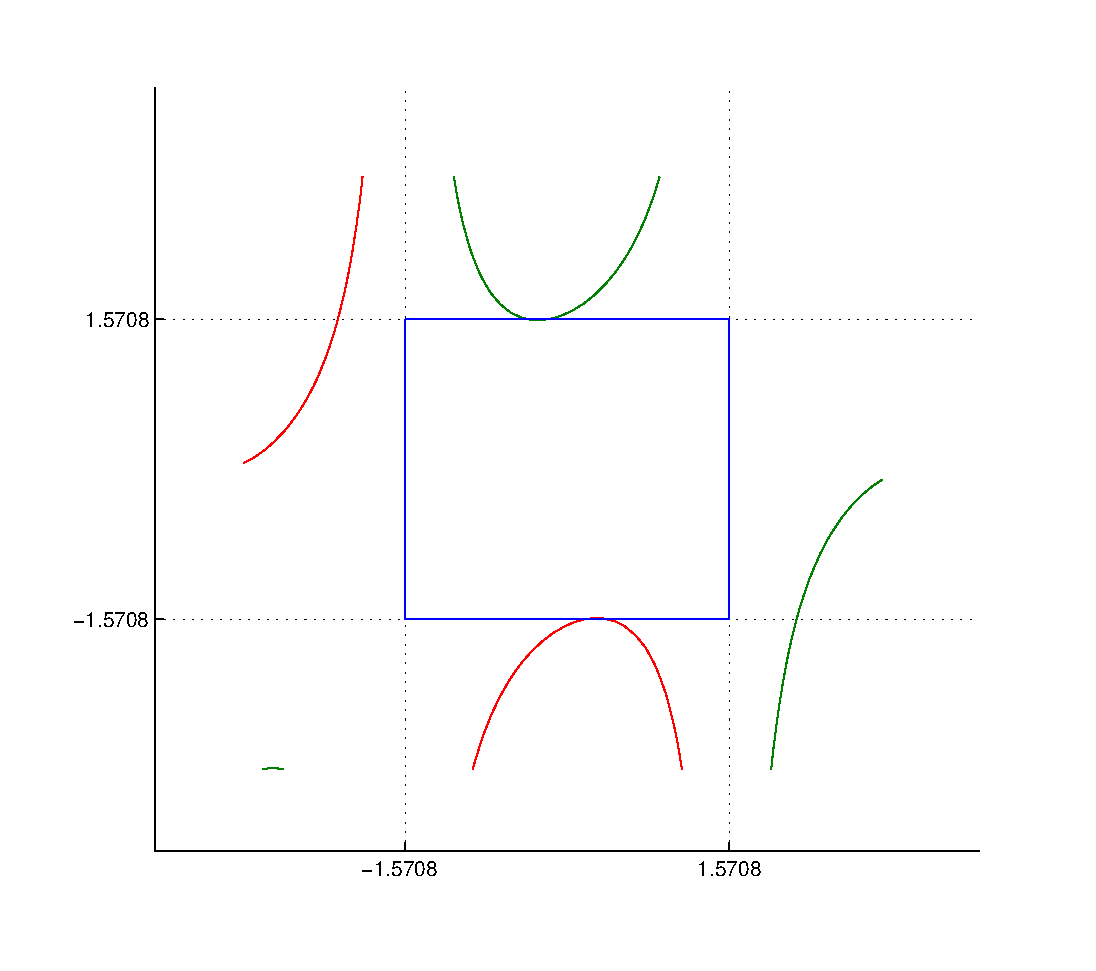
\includegraphics[width=10cm]{phik_hk_ex_LPJ12}
	\caption{Região $\Phi_k$ limitada por $\dot{h}_k$, $\Phi_k$ é apresentado em azul, $\dot{\alpha}_1$ em vermelho e $\dot{\alpha}_2$ em verde}
	\label{fig:hk_phik}
\end{figure}

A Figura \ref{fig:hk_phik} mostra a região $\Phi_k$ limitada pela variação das funções de pertinência do modelo fuzzy T-S para o Exemplo\ref{sec:ex2_JPJ12_again}, considerando-se toda a região de modelagem $C$. Para se obter $\Phi_k$, primeiramente derivaram-se as funções de associação $\alpha_1$ e $\alpha_2$ do sistema, as quais equivalem a, respectivamente,
\begin{equation}\label{eq:func_assoc_LPJ12}
\alpha_1(x) = \alpha_1(z(t)) = \dfrac{1+\sin(x_1(t))}{2}\qquad \alpha_2(x) = \alpha_2(z(t)) = 1 - \alpha_1(z(t))
\end{equation}
A variação de $\alpha_k$ é dada segundo a relação a seguir, considerando a regra da cadeia para derivadas.
\begin{equation}\label{eq:diff_alpha}
\dot{\alpha}_k(x) = \dfrac{d\alpha_k(x)}{dx} \dot{x}.
\end{equation}
Considerando o modelo não linear do sistema, tem-se que $\dot{x} = Ax$, substituindo essa igualdade na Equação \ref{eq:diff_alpha}, temos que
\begin{equation}\label{eq:diff_alpha}
\dot{\alpha}_k(x) = \dfrac{d\alpha_k(x)}{dx} \dot{x}.
\end{equation}
Sabendo que o modelo não linear do Exemplo em questão é dado por
\begin{equation*}
\mathbf{\dot{x} = \begin{bmatrix} -2 & 4\\  -1 - \dfrac{\lambda (1 - sen(x_1))}{2} & -2 \end{bmatrix}x_1}
\end{equation*}
Então, tem-se que
\begin{equation}\label{eq:dot_h_1}
\dot{\alpha}_1 = \dfrac{\cos(x_1)}{2}(-2x_1+4x_2)
\end{equation}
\begin{equation}\label{eq:dot_h_2}
\dot{\alpha}_2 = \dfrac{\cos(x_1)}{2}(-1-\dfrac{\lambda (1-\sin(x_1))}{2})x_1-2x_2)
\end{equation}

Para obter os valores máximos e mínimos das variações de $\alpha_k$, variou-se $x_1$ e $x_2$ dentro da faixa de valores definidos para estes em $C$, com $\alpha_{1_{min}} = \alpha_{2_{min}} = 0$ e $\alpha_{1_{max}} = \alpha_{2_{max}} = 3.2657$. Observe que, se plotada em torno da origem, a região de $\Phi_k$ equivale a $C$.

Para este valor de $\Phi_k$ máximo, para $\lambda = 20$ e para o modelo fuzzy T-S obtido para o setor local $C$, as LMIs do Teorema \ref{th:theorem_6} não geraram solução, de forma que se conclui que a origem do sistema não é estável para esta região. Reduzindo-se a região de definição do sistema gradativamente, tal que se diminui-se o valor de $\Phi_k$ da mesma maneira, obteve-se que o sistema é instável para $\lambda = 20$ somente para a regiões menores ou iguais a $0.51C$.

Para este método em especial, além do parâmetro $\lambda$ que pode ser variado, a análise da estabilidade do sistema depende também de $\Phi_k$, pois este pode ser variado dentre a faixa de valores máximo e mínimo obtido da variação das $h_k$, que por sua vez variam para cada região contida em $C$. Desta maneira, o procedimento adotado para se obter os limites superiores e inferiores de $\lambda$ consistirá em variar a região limitada por $\dot{h}_k$, resolvendo-se as Equações \ref{eq:dot_h_1} e \ref{eq:dot_h_2} para regiões cada vez menores contidas em $C$, de forma a se obter um valor diferente de $\Phi_k$ e assim obter os valores máximos e mínimos de $\lambda$ para cada um dos valores de $\Phi_k$.

Como sabe-se que $\Phi_k$ está contido no intervalo $[0, \pi]$, pois foram os valores obtidos para o melhor caso, em que se considera toda a região $C$, pode-se assumir esta faixa de valores, sem se precisar resolver novamente $\dot{h}_k$, para se obter os valores máximos e mínimos de $\lambda$ para cada valor de $\Phi_k$.

Logo, primeiramente definiu-se $\Phi_k = 0.1$ e variou-se $\lambda$ a partir de $0$, em passos de $0.1$, até o valor máximo para o qual o sistema permanecesse estável. Em seguida aumento-se $\Phi_k$ em passos de 0.1 e obtiveram-se os valores máximos de $\lambda$ para os quais se manteve a condição para estabilidade. Para cada valor de $\Phi_k$ obteve-se um limitante superior de $\lambda$ diferente para a estabilidade. De forma análoga obtiveram-se os limitantes de $\lambda$ para cada valor de $\Phi_k$, com a diferença de que a variação dos valores $\lambda$ a partir de $0$ foi feita em passos de $-0.1$.

Verificou-se o valor mínimo de $\lambda$ para o qual a origem permanece como um ponto de estabilidade do sistema para qualquer valor de $\Phi_k$ é igual a $-1.9$. Já o valor máximo de $\lambda$ tal que se garanta a estabilidade varia conforme $\Phi_k$ varia, de forma que se obteve a curva que relaciona estas duas grandezas, conforme mostra a Figura \ref{fig:phi_k_vs_lambda_max}.

\begin{figure}[htbp]
	\centering
	\includegraphics[width=10cm]{phi_vs_lambda_max}
	\caption{$\lambda_{max}$ versus $\Phi_k$}
	\label{fig:phi_k_vs_lambda_max}
\end{figure}

\subsubsection{Método 3: (Método Proposto) Função Lyapunov com $P$ dependente das funções de pertinência e Teorema \ref{th:main_result}}

Ao se utilizar o Teorema \ref{th:main_result}, para verificar se o ponto de equilíbrio na origem é um ponto localmente estável, será necessário obter solução das condições apresentadas neste teorema.

De forma genérica, $P(\alpha)$ é constituído pelo conjunto das matrizes vértices $P_i$, constantes e simétricas, associadas a cada um dos $r$ termos do primeiro simplex $\alpha$, em que $r$ é o número de regras do modelo fuzzy T-S, tais que
\begin{equation}\label{eq:P_alpha}
P(\alpha) = \sum_{i = 1}^{r}\alpha_iP_i
\end{equation}
A matriz $A(\alpha)$ consiste no somatório dos vértices do modelo fuzzy Takagi-Sugeno associados a cada um dos $r$ termos do primeiro simplex, conforme apresentado a seguir.
\begin{equation}\label{eq:A_alpha_eq}
A(\alpha) = \sum_{i = 1}^{r}\alpha_iA_i
\end{equation}
Analogamente, a matriz $X(\alpha)$ é obtida pela combinação de $r$ vértices $X_i$ constantes, mas que não precisam ser simétricos, em função do primeiro simplex $\alpha$.
\begin{equation}\label{eq:X_alpha}
X(\alpha) = \sum_{i = 1}^{r}\alpha_iX_i
\end{equation}
Desta maneira, obtemos para o exemplo em discussão $P(\alpha)$, $X(\alpha)$ e $A(\alpha)$, respectivamente, conforme segue
\begin{equation*}
\begin{array}{lcl}
P(\alpha) & = & \alpha_1P_1 + \alpha_2P_2\\
X(\alpha) & = & \alpha_1X_1 + \alpha_2X_2\\
A(\alpha) & = & \alpha_1\begin{bmatrix}-2&4\\-1&-2\end{bmatrix} + \alpha_2\begin{bmatrix}-2&4\\-(1+\lambda)&-2\end{bmatrix}
\end{array}
\end{equation*}
em que $P_i$ e $X_i, i = 1, 2$  são matrizes $2 \times 2$, correspondentes aos parâmetros a se obter para a análise de estabilidade.

Para obter $J(\theta)$, devemos primeiramente obter as jacobianas de $\alpha = \begin{bmatrix}\alpha_1\\\alpha_2\end{bmatrix}$ em relação a $x = \begin{bmatrix}x_1\\x_2\end{bmatrix}$, as quais correspondem a
\begin{equation*}
\dot{\alpha} = \nabla_x\alpha
\end{equation*}
Assim,
\begin{equation*}
J(x) = \begin{bmatrix}\dot{\alpha}_1\\\dot{\alpha}_2\end{bmatrix}= \begin{bmatrix}\frac{\partial \alpha_1}{\partial x_1}&\frac{\partial \alpha_1}{\partial x_2}\\\frac{\partial \alpha_2}{\partial x_1}&\frac{\partial \alpha_2}{\partial x_2}\end{bmatrix}
= \begin{bmatrix}\dfrac{\cos(x_1)}{2}&0\\\dfrac{-\cos(x_1)}{2}&0\end{bmatrix}
\end{equation*}

Os vértices $J_i$ oriundos de $J(x)$ são obtidos a partir de todas as combinações dos valores limitantes superiores e inferiores de todos os termos dependentes de $x$. É possível identificar que o único termo dependente de $x$ em $J(x)$ é $\cos(x_1)$, que, para a região $C$, tem seus valores máximos e mínimos equivalentes a 1 e 0, respectivamente. Assim, encontramos dois vértices de $J(x)$, os quais são
\begin{equation*}
J_1 = \begin{bmatrix}0&0\\0&0\end{bmatrix}\qquad J_2 = \begin{bmatrix}1&0\\1&0\end{bmatrix}
\end{equation*}
Desta maneira, obtemos $J(\theta)$ como sendo
\begin{equation*}
J(\theta) = \theta_1\begin{bmatrix}0&0\\0&0\end{bmatrix} + \theta_2\begin{bmatrix}1&0\\1&0\end{bmatrix}
\end{equation*}
Como já visto, o sistema possui dois vértices em $P$, os quais são $P_1$ e $P_2$. Além disso, o poliédro em função dos vértices que representa a região $C$ de modelagem do sistema fuzzy T-S é dado por
\begin{equation*}
\chi = co\begin{Bmatrix}x^1,x^2,x^3,x^4\end{Bmatrix} = co\begin{Bmatrix}
\begin{bmatrix}-\pi/2\\-\pi/2\end{bmatrix},\begin{bmatrix}-\pi/2\\\pi/2\end{bmatrix},\begin{bmatrix}\pi/2\\-\pi/2\end{bmatrix},\begin{bmatrix}\pi/2\\\pi/2\end{bmatrix}
\end{Bmatrix}
\end{equation*}
A partir disso, podemos obter $Q(\gamma)$, o qual possui $4$ vértices, conforme a quantidade de vértices de $\chi$, conforme segue.
\begin{equation*}
Q(\gamma) = \gamma_1\begin{bmatrix}P_1x^1&P_2x^1\end{bmatrix}+\gamma_2\begin{bmatrix}P_1x^2&P_2x^2\end{bmatrix}+\gamma_3\begin{bmatrix}P_1x^3&P_2x^3\end{bmatrix}+\gamma_4\begin{bmatrix}P_1x^4&P_2x^4\end{bmatrix}
\end{equation*}

Obtidos todos os termos da LMI \ref{eq:th1_stability}, estaríamos prontos para resolvê-la. Porém, para se obter a solução correta da LMI, considerando os três simplexes $\alpha$, $\theta$ e $\gamma$, é preciso colocar todos os termos da LMI em função de todos os simplexes, isto porque as ferramentas utilizadas para resolver as LMIs neste trabalho não permitem a solução de LMI com termos dependentes de simplexes diferentes entre si.

Na Equação \ref{eq:P_alpha}, por exemplo, temos que $P(\alpha)$ é dependente do primeiro simplex $\alpha$, o grau de relação de $\alpha$ com os vértices de $P(\alpha)$ é de ordem 1. Podemos representar $P(\alpha)$ também em função dos demais simplexes $\theta$ e $\gamma$, sem que haja perda de generalidade, uma vez que $\sum_{i = 1}^{\vartheta}\theta_i = 1$ e $\sum_{i = 1}^{\Gamma}\gamma_i = 1$, da mesma maneira que $\sum_{i = 1}^{r}\gamma_i = 1$. Assim,
\begin{equation}\label{P_multiple_simplexes}
P(\alpha) = \sum_{i = 1}^{r}\alpha_iP_i = P(\alpha, \theta,\gamma) = \sum_{i = 1}^{r}\alpha_i\sum_{i = j}^{\vartheta}\theta_j\sum_{k = 1}^{\Gamma}\gamma_kP_i
\end{equation}

Portanto, para que $ P(\alpha, \theta,\gamma)$ equivalha a $P(\alpha)$, basta assumir o grau de $\theta$ e $\gamma$ como sendo igual a 0 para este termo. Seguindo este mesmo procedimento, encontramos todos os demais elementos da LMI em função de todos os três simplexes do sistema. Agora, finalmente, as LMIs do Teorema \ref{th:main_result} podem ser resolvidas para verificar se o sistema é estável segundo esta abordagem para a região de validade do sistema $C$.

Este método permitiu verificar que o sistema é estável na região $C$ para $\lambda = 20$.

Assim como se fez para os demais métodos, é possível obter os limitantes superiores e inferios de $\lambda$ para os quais o sistema permanece estável para a região $C$ na qual os estados do sistema são válidos e para as quais o modelo fuzzy Takagi-Sugeno fora obtido.

Observou-se que para este método não há um limitante superior de $\lambda$ para o qual a origem se torne instável na região $C$. Por outro lado, valor mínimo de $\lambda$ tal que a origem se mantém estável equivale a $-0.8000$.

\subsubsection{Comparação entre os métodos}

Na Seção \ref{sec:resultado_principal} foi apresentado o resultado principal deste trabalho, que consiste na formulação de um novo método para determinação de estabilidade de sistemas não lineares modelados como sistemas fuzzy Takagi-Sugeno utilizando-se a teoria de estabilidade de Lyapunov via LMIs. A proposta desta seção é comparar o método proposto com outros métodos, a fim de se verificar se essa nova técnica de obtenção de estabilidade é realmente mais relaxada que demais técnicas propostas na literatura. Estes outros métodos da literatura correspondem aos Métodos 1 e 2 apresentados acima. A comparação entre os métodos será feita com base na obtenção dos resultados da aplicação de cada um destes métodos no Exemplo \ref{example_LPJ12}, que é dependente do parâmetro $\lambda$. 

O critério para se determinar qual o melhor método consiste, primeiramente, na verificação de qual método garante a estabilidade assintótica para a maior região do espaço de estados, sendo este o método a ser considerado menos conservador. Em seguida, será feita a comparação  entre os valores máximo e mínimo de $\lambda$ obtidos por cada método para os quais o sistema permanece estável. Este critério de comparação é baseado em na referência bibliográfica \cite{MPSM:2009}.


Nesta seção pôde-se comparar o método de análise de estabilidade de Lyapunov via LMIs aqui proposto com outros métodos já existentes na literatura. Utilizou-se dois métodos para este procedimento, o primeiro método consistiu na análise de estabilidade considerando-se $P$ constante, segundo proposto por (Boyd, 1994 \cite{bookboydl:1994}), o segundo método foi proposto por (Mozelli, Palhares, Sousa e Mendes, 2009 \cite{MPSM:2009}) e nele se considera $P(\alpha)$ e limitante simples das derivadas. Além disso, nomeou-se o método introduzido neste trabalho como Método 3.

Fixando-se $\lambda$ = 20, observou-se que os Métodos 1 e 2 não garantem a estabilidade do sistema para toda a região $C$ para a qual o sistema é definido; ao contrário do Método 3, que garante estabilidade para esta região e este valor de $\lambda$. O Método 1 só garante estabilidade para $\lambda = 20$ para regiões menores ou iguais $0.46C$, enquanto que para o Método 2 o sistema já apresenta valores estáveis para regiões menores ou iguais a $0.51C$.

A busca pelos valores máximo e mínimo de $\lambda$ para os quais o sistema é estável considerando toda a região $C$ permitiu verificar qual dentre os três métodos gera melhores resultados. Para o limitante superior de $\lambda$, verificou-se que o Método 3 garante estabilidade para seja qual for o valor de $\lambda_{max}$, enquanto o Método 1 se limita a $\lambda_{max} = 9.6000$ e o Método 2, para o melhor caso, em que $\Phi_k$ é mínimo, é limitado em $\lambda_{max} = 214.7000$. Assim, o Método 3 gera os melhores resultados para a estabilidade do ponto de equilíbrio na origem, considerando o limitante superior de $\lambda$.

Para o limitante inferior de $\lambda$, obteve-se que os Métodos 1 e 2 são estáveis na região $C$ para valores de $\lambda_{min}$ maiores ou iguais a $-1.9000$. O Método 3, por sua vez, garante a estabilidade apenas para $\lambda \geq -0.8000$. Logo, o Método 3 gera o pior resultado para o limitante inferior de $\lambda$.

\subsection{Exemplo Sistema {\it Droop}}

Uma vez comprovado que o método proposto nos resultados principais provê o melhor resultado para a análise de estabilidade de sistemas dinâmicos, quando comparado com os Métodos 1 e 2, e para $\lambda > 0$, este método será utilizado para a análise de estabilidade de sistemas com dinâmica fuzzy T-S.

Nesta seção serão apresentados os resultados de análise de estabilidade dos Exemplos \ref{ex:droop_UFSM_fuzzyTS} e \ref{ex:4_tanques}, que equivalem, respectivamente ao sistema do inversor de tensão e ao processo de quatro tanques vistos no capítulo anterior.

\begin{example}[Sistema {\it Droop}] \label{ex:estab_sist_droop}
No Exemplo \ref{ex:droop_UFSM_fuzzyTS} foi apresentada a modelagem fuzzy T-S do sistema do inversor de tensão, agora será feita a análise de estabilidade deste sistema, utilizando o modelo proposto no Teorema \ref{th:main_result}. Será verificado se o sistema é estável para a região definida por $C = \{x(t) \in \rm I\!R^3 | x_1(t) = P_f \in [0; 25000], x_2(t) = Q_f \in [-70000; 5000], x_3(t) = \delta \in [-0.02; 0.1]\}$.
\end{example}

Para tanto, é preciso encontrar uma solução para as LMIs propostas no Teorema \ref{th:main_result}, de forma que obtenha $P > 0$. Os parâmetros da LMI\ref{eq:th1_stability} para este exemplo são obtidos conforme segue.

Sabendo-se que o modelo fuzzy T-S do sistema possui 16 vértices $A_i$ e 16 fun\~{c}ões de associação $\alpha_i, i = 1, \hdots, 16$, com $A_i$ e $\alpha_i$ obtidos no capítulo anterior,$A(\alpha)$ é dado por
\begin{equation*}
A(\alpha) = \sum_{i = 1}^{16}\alpha_iA_i
\end{equation*}
De forma análoga, $P(\alpha)$ é obtido como
\begin{equation*}
P(\alpha) = \sum_{i = 1}^{16}\alpha_iP_i
\end{equation*}
Em que $P_i, i = 1,\hdots, 16$ são matrizes simétricas a serem determinadas. $X_i, i = 1,\hdots,16$ também são matrizes, porém náo simétricas a serem determinadas, tais que
\begin{equation*}
X(\alpha) = \sum_{i = 1}^{16}\alpha_iX_i
\end{equation*}
Para obter o termo $J(\theta)$, primeiramente é preciso obter as jacobianas de $\alpha$. Por possuir 16 regras fuzzy, o que resulta em 16 funções de pertinência, e por possuir três vairáveis de estado, a jacobiana $J$ será uma matriz de dimensão $16 \times 3$. O termo $J(\theta)$ terá $2^m$ \v{e}rtices, em que $m$ é o número de não linearidades da jacobiana J.

A função de pertinência $\alpha_1$, por exemplo, equivale a
\begin{equation*}
\alpha_1(z) = M_{11}M_{12}M_{13}M_{14}
\end{equation*}
Neste exemplo, os graus de pertinência são dependentes unicamente do estado $x_3$. Assim, a jacobiana de $\alpha_1$ será dada por
\begin{equation*}
\alpha_1(z) = \begin{bmatrix}0&0&\frac{\partial\alpha_1(z)}{\partial x_3}\end{bmatrix}
\end{equation*}
Em que 
\begin{equation*}
\frac{\partial\alpha_1(z)}{\partial x_3} = \dot{M}_{11}M_{12}M_{13}M_{14}+M_{11}\dot{M}_{12}M_{13}M_{14}+M_{11}M_{12}\dot{M}_{13}M_{14}+M_{11}M_{12}M_{13}\dot{M}_{14}
\end{equation*}
Os graus de pertinência $M_{ij}$ são dados por
\begin{equation*}
M_{1i} = \dfrac{z_i-min(z_i)}{\Delta z_i}\qquad M_{2i}= 1 -  M_{1i}
\end{equation*}
Assim,
\begin{equation*}
\dot{M}_{1i} = \dfrac{\dot{z_i}}{\Delta z_i} = -\dot{M}_{2i}
\end{equation*}
Sabendo-se que
\begin{equation*}
z_1 = \cos(x_3) \Rightarrow \dot{z}_1 = -\sin(x_3)\qquad z_3 = \sin(x_3) \Rightarrow \dot{z}_3 = \cos(x_3)
\end{equation*}
Logo tem-se que
\begin{equation*}
\dot{z}_1 = -z_3\quad\text{e}\quad\dot{z}_3 = z_1
\end{equation*}
Das relações acima, tem-se que
\begin{equation*}
\dot{M}_{11}= -\dfrac{\dot{z_3}}{\Delta z_1}
\end{equation*}
Como
\begin{equation*}
{M}_{13}= -\dfrac{z_3-min(z_3)}{\Delta z_3}\Rightarrow z_3 = {M}_{13}\Delta z_3+min(z_3)
\end{equation*}
Logo,
\begin{equation*}
\dot{M}_{11} = -{M}_{13}\dfrac{\Delta z_3}{\Delta z_1}-\dfrac{min(z_3)}{\Delta z_1}
\end{equation*}
De forma análoga,
\begin{equation*}
\dot{M}_{13} = {M}_{11}\dfrac{\Delta z_1}{\Delta z_3}-\dfrac{min(z_1)}{\Delta z_3}
\end{equation*}
Assim, $\dot{\alpha}_i(z)$ pode ser reescrito como

\begin{align*}
\frac{\partial\alpha_1(z)}{\partial x_3} &= (-{M}_{13}\dfrac{\Delta z_3}{\Delta z_1}-\dfrac{min(z_3)}{\Delta z_1})M_{12}M_{13}M_{14}+M_{11}\dot{M}_{12}M_{13}M_{14}\\
&+ M_{11}M_{12}({M}_{11}\dfrac{\Delta z_1}{\Delta z_3}-\dfrac{min(z_1)}{\Delta z_3})M_{14}+M_{11}M_{12}M_{13}\dot{M}_{14}
\end{align*}
Assim, é possível verificar que $\frac{\partial\alpha_1(z)}{\partial x_3}$ é dependente de 6 termos não lineares, os quais são
\begin{equation*}
M_{11}, M_{12}, M_{13}, M_{14}, \dot{M}_{12}, \dot{M}_{14}
\end{equation*}

As demais derivadas parciais de $\alpha$ são obtidas com base nos mesmos princípios, obtendo-se os mesmos termos não lineares de $\alpha_1$.

Finalmente, como os vértices de $J(\theta)$ são dependentes de 6 termos não lineares distintos, foram obtidos os 64 vértices de $J(\theta)$, oriundos de todas as combinações possíveis dos valores máximos e mínimos das não linearidades de J.

Para a obtenção do termo $Q(\gamma)$ é preciso primeiramente obter a representação por vértices do poliédro $\chi$ contido na região limitada pelos valores máximos e mínimos das variáveis de estado. Assim, obtém-se
\begin{align*}
\chi &= co\begin{Bmatrix}x^1,x^2,x^3,x^4,x^5,x^6,x^7,x^8\end{Bmatrix}\\
 &= co\begin{Bmatrix}
\begin{bmatrix}0\\-70000\\-0.02\end{bmatrix}, \begin{bmatrix}0\\-70000\\ 0.1\end{bmatrix}, \begin{bmatrix}0\\5000\\ 0.1\end{bmatrix}, \begin{bmatrix}0\\5000\\ -0.02\end{bmatrix}, \begin{bmatrix}25000\\-70000\\-0.02\end{bmatrix}, \begin{bmatrix}25000\\-70000\\ 0.1\end{bmatrix}, \begin{bmatrix}25000\\5000\\ 0.1\end{bmatrix}, \begin{bmatrix}25000\\5000\\ -0.02\end{bmatrix}
\end{Bmatrix}
\end{align*}
O parâmetro $Q(\gamma)$, portanto, terá 8 vértices, dados por

\begin{equation*}
Q(\gamma) = \gamma_1\begin{bmatrix}P_1x^1&P_2x^1&\hdots&P_16x^1\end{bmatrix}+\gamma_2\begin{bmatrix}P_1x^2&P_2x^2&\hdots&P_16x^2\end{bmatrix}+\hdots+\gamma_8\begin{bmatrix}P_1x^8&P_2x^8&\hdots&P_{16}x^8\end{bmatrix}
\end{equation*}


Obtidos todos os termos das LMIs de análise de estabilidade do Teorema \ref{th:main_result}, é necessário colocá-los em função dos três simplexes $\alpha$, $\theta$ e $\gamma$, o que foi feito conforme mostrou a Equação \ref{P_multiple_simplexes}.

Resolvendo-se as LMIs do Teorema \ref{th:main_result}, verificou-se que o sistema é estável para a região $C$ para a qual foi definido.

\section{Considerações Finais}

Neste capítulo foi proposto um novo método para determinação de estabilidade de Lyapunov via LMIs de sistemas dinâmicos não lineares como sistemas fuzzy Takagi-Sugeno pelo método de não linearidade de setor. Foi proposto o Teorema \ref{th:main_result}, para o qual esperou-se obter resultados menos conservadores para a análise de estabilidade do sistema. O Exemplo \ref{example_LPJ12} foi utilizado para a aplicação do Teorema proposto. Verificou-se, por meio deste teorema, que a origem é um ponto de equilíbrio estável, considerando-se $\lambda = 20$, para toda a região $C$ para a qual os estados do sistema são definidos.

Para se este método é, de fato, menos conservador que outros métodos existentes na literatura, foi realizada a análise de estabilidade deste mesmo sistema por meio de outros dois métodos. O primeiro dentre estes Métodos consistiu utilização do método de Lyapunov para $P$ constante e dinâmica fuzzy T-S. Para este método, verificou-se que a origem somente é um ponto estável do sistema, com $\lambda = 20$, para regiões menores ou iguais a $0.46C$, em que $C$ é a região de validade do sistema no plano de estados.

O segundo método consistiu na análise de estabilidade para o sistema com $P$ dependente das funções de associação $\alpha$ do modelo fuzzy T-S, porém considerando-se a configuração por limitantes simples das derivadas, conforme proposto na referência \cite{MPSM:2009}. Pra este método, verificou-se o que, para $\lambda = 20$, a origem somente é um ponto de equilíbrio estável para regiões menores ou iguais a $0.51C$.

Utilizando-se o critério da região para a qual o ponto de equilíbrio é estável para cada método, como o Teorema proposto neste capítulo garantiu a estabilidade para uma região maior que os demais, verificou-se que este método é de fato mais relaxado.

Outro parâmetro de comparação utilizado foi, fixando-se a região $C$ de validação, qual seriam os valores de $\lambda$ máximo e mínimo para os quais o sistema seja estável nesta região do plano de estados. Verificou-se que para o limitante inferior, o Teorema \ref{th:main_result} produziu o pior resultado, já que deixou de ser estável para um valor maior de $\lambda$ quando comparado com os demais métodos, uma vez que obteve $min(\lambda) = -0.8000$, enquanto os demais métodos apresentaram $min(\lambda) = -1.9000$. Por outro lado, o Teorema \ref{th:main_result} se mostrou ser o melhor método para a determinação da estabilidade, uma vez que não fora encontrado limitante superior de $\lambda$ a partir de qual a origem deixasse de ser um ponto de equilíbrio assintoticamente estável.